\documentclass[11pt]{article}

\usepackage[a4paper,margin=1in]{geometry}
\usepackage{amsmath,amssymb}
\usepackage{booktabs}
\usepackage{fancyhdr}
\usepackage{pgfplots}
\usepackage{pgfplotstable}
\usepackage{xcolor}
\usepackage{verbatim}
\usepackage{listings}
\usepackage[hidelinks]{hyperref}

\pgfplotsset{compat=1.18}
\setlength{\parindent}{0pt}
\setlength{\parskip}{0.6em}
\setlength{\headheight}{13.6pt}

\pagestyle{fancy}
\fancyhf{}
\lhead{Applied Data Analysis}
\rhead{Worked Notes}
\cfoot{\thepage}

\definecolor{navy}{HTML}{23395D}
\definecolor{teal}{HTML}{2A9D8F}
\definecolor{orange}{HTML}{C45824}
\definecolor{codebg}{HTML}{F5F7FA}
\lstdefinestyle{rcode}{
    basicstyle=\ttfamily\scriptsize,
    backgroundcolor=\color{codebg},
    frame=single,
    rulecolor=\color{navy!30},
    breaklines=true,
    columns=fullflexible,
    keepspaces=true,
    showstringspaces=false,
    tabsize=2
}

\begin{document}

\begin{center}
{\Large Applied Data Analysis}\\[0.3em]
{\large Worked Notes}\\[0.3em]
{\normalsize Victoria apartment investment recommendation}
\end{center}

\section*{Worked report}

\subsection*{1) Data summary}
The three datasets were merged by \texttt{Suburb\_name}. Each source file contained 458 suburbs, with no duplicate suburb names, and the inner join retained all 458 suburbs, so no rows were lost in the merge. Several data quality issues were then corrected before modelling. In \texttt{d01.csv}, \texttt{NORLANE} had the value \texttt{309334x}, so the numeric part was parsed as 309,334 rather than deleting an otherwise valid row. \texttt{POINT LONSDALE} had missing historical median income and was imputed using the historical income median, which is robust to skew; no other column contained missing values. Unemployment rates cannot be negative, so 22 historical and 22 projected negative observations were capped at zero, preserving the low-unemployment signal. The price histogram below made the strong right skew and one extreme value obvious: \texttt{MAFFRA} recorded a median apartment price of 4,202,660, far above the next highest suburb, so it was treated as an outlier and excluded from the regression training sample. The remaining graphs show the positive association between population growth and price, and the final predicted top suburbs.

\subsection*{2) Model Estimation}
I estimated the relationship between historical suburb characteristics and 2023 apartment prices with the following linear regression:
\[
\begin{aligned}
\log(\text{Price}_{2023})=&
\beta_0+\beta_1\text{PopulationGrowth}+\beta_2\text{Income10k}\\
&+\beta_3\text{UnemploymentClean}+\beta_4\text{PriorityArea}+\varepsilon.
\end{aligned}
\]
The dependent variable is log median apartment price. The log transformation is appropriate because prices are positive and right-skewed, and it makes coefficients interpretable as approximate percentage changes. \texttt{Income10k} equals median income divided by 10,000, so its coefficient describes the effect of an additional 10,000 dollars of income. The training sample contains 457 suburbs after excluding \texttt{MAFFRA}. The model has \(R^2=0.523\), so it explains about 52.3\% of the variation in log prices across suburbs.

\begin{center}
\begin{tabular}{lrrrr}
\toprule
Variable & Coef. & Std. err. & t & approx. p \\
\midrule
Intercept & 11.333 & 0.080 & 140.89 & 0.0000 \\
Population growth & 0.288 & 0.013 & 21.86 & 0.0000 \\
Income per \$10k & 0.006 & 0.003 & 1.86 & 0.0628 \\
Cleaned unemployment & -0.036 & 0.004 & -8.90 & 0.0000 \\
Priority growth area & 0.380 & 0.035 & 10.74 & 0.0000 \\
\bottomrule
\end{tabular}
\end{center}

\subsection*{3) Model interpretation}
Population growth is positive and statistically strong: a one percentage point increase in historical population growth is associated with about \(e^{0.288}-1=33.4\%\) higher prices, holding the other variables fixed. Cleaned unemployment is negative: a one percentage point increase in unemployment is associated with about 3.6\% lower prices. Priority growth area is also economically meaningful; the coefficient of 0.380 implies a predicted price premium of about \(e^{0.380}-1=46.2\%\). Income is positive but weaker statistically, so it should not be over-interpreted.

Using the projected demographic data as next-year feature data, \texttt{DROUIN} has the highest predicted price level: 992,801 compared with its current 667,824, a predicted uplift of 48.7\%. However, I recommend \texttt{SEAFORD} as the stronger investment case. Its predicted price is 951,068, and its uplift from the current 490,411 is 93.9\%. It also has very high projected population growth of 8.86\%, so the recommendation is not based only on a low starting price.

On the Gauss-Markov assumptions, the main concern is exogeneity: omitted variables such as transport, schools, development constraints and suburb amenities are likely correlated with the included regressors, which can bias the estimated coefficients. The wide spread of prices across suburbs also suggests possible heteroskedasticity, so the reported standard errors should be read with some caution. For these reasons the regression should be interpreted as association rather than causal proof, and the predictions treated as a guide to be combined with local due diligence.

\section*{Supporting graphs}

\begin{figure}[h!]
\centering
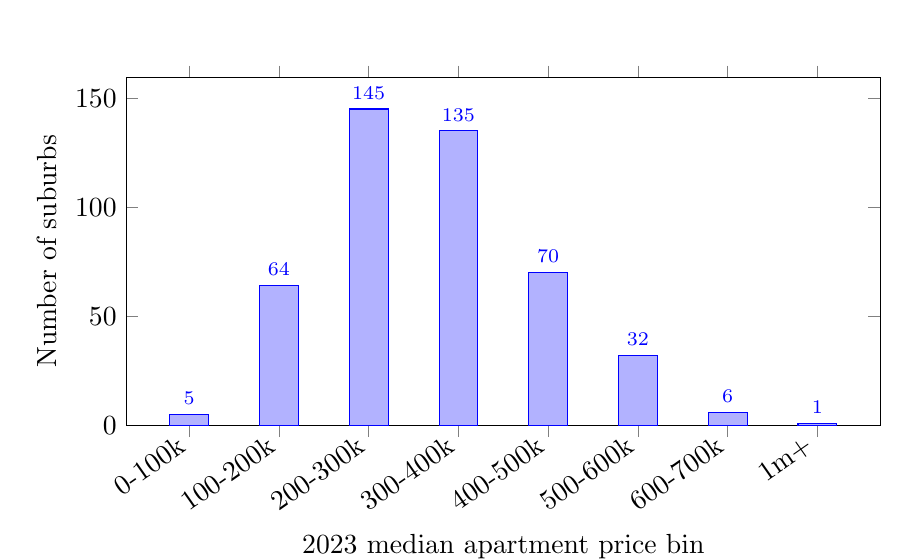
\begin{tikzpicture}
\begin{axis}[
    ybar,
    width=0.92\textwidth,
    height=6cm,
    xlabel={2023 median apartment price bin},
    ylabel={Number of suburbs},
    symbolic x coords={0-100k,100-200k,200-300k,300-400k,400-500k,500-600k,600-700k,1m+},
    xtick=data,
    x tick label style={rotate=35,anchor=east},
    ymin=0,
    bar width=14pt,
    nodes near coords,
    nodes near coords style={font=\scriptsize},
    fill=teal
]
\addplot coordinates {(0-100k,5) (100-200k,64) (200-300k,145) (300-400k,135) (400-500k,70) (500-600k,32) (600-700k,6) (1m+,1)};
\end{axis}
\end{tikzpicture}
\caption{The price distribution is right-skewed and contains a clear extreme outlier above 1 million.}
\end{figure}

\begin{figure}[h!]
\centering
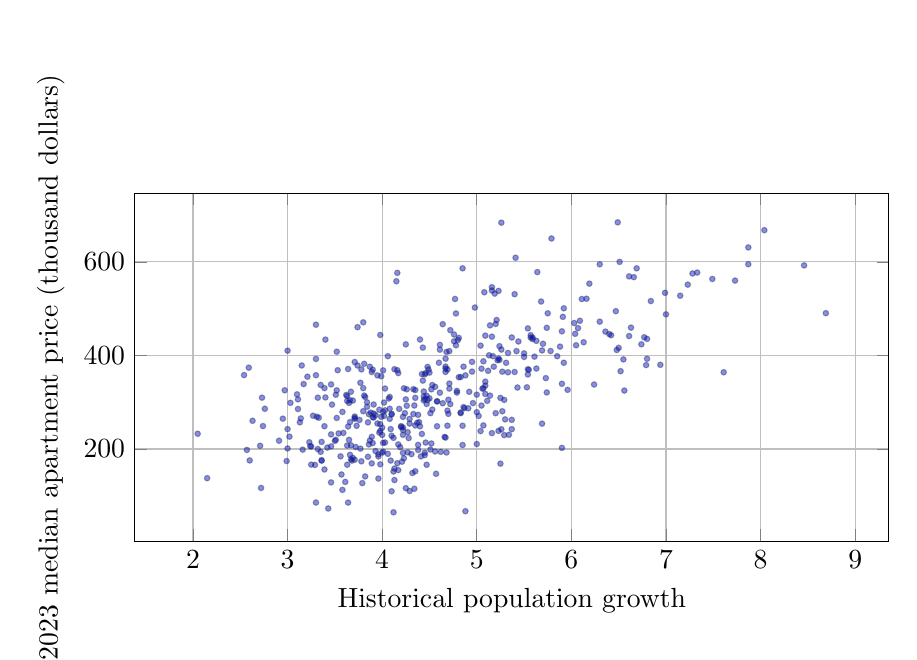
\begin{tikzpicture}
\begin{axis}[
    width=0.92\textwidth,
    height=6cm,
    xlabel={Historical population growth},
    ylabel={2023 median apartment price (thousand dollars)},
    grid=major,
    mark size=1pt,
    only marks
]
\addplot+[only marks, mark=*, color=navy, opacity=0.45] coordinates {
(3.240,206.2)
(4.430,416.8)
(4.570,147.1)
(6.550,391.5)
(8.040,667.8)
(4.530,284.4)
(2.590,373.9)
(4.980,502.4)
(4.290,264.4)
(2.970,325.6)
(3.860,274.5)
(3.930,195.7)
(3.500,217.4)
(3.110,285.6)
(3.390,156.3)
(4.780,489.8)
(6.160,521.2)
(6.040,446.2)
(4.510,276.7)
(5.610,397.5)
(4.120,223.9)
(4.250,116.4)
(7.150,527.7)
(5.630,431.2)
(6.490,684.5)
(3.910,275.8)
(5.250,309.3)
(3.630,207.5)
(5.290,305.0)
(3.910,295.2)
(4.420,232.3)
(4.390,257.6)
(4.090,242.6)
(3.510,219.7)
(4.350,152.5)
(3.760,262.2)
(4.230,180.4)
(3.000,201.3)
(3.400,310.3)
(3.300,465.7)
(4.310,189.2)
(4.030,214.0)
(3.650,219.7)
(5.300,263.4)
(4.710,409.3)
(4.830,278.1)
(7.230,551.4)
(5.070,250.5)
(2.630,260.4)
(5.420,409.3)
(4.610,320.5)
(4.520,327.7)
(5.270,365.3)
(3.270,271.2)
(5.260,412.5)
(5.540,457.9)
(3.930,272.7)
(4.270,193.1)
(4.000,245.7)
(5.690,410.8)
(4.610,412.4)
(4.080,286.1)
(3.980,253.2)
(3.780,173.8)
(6.130,428.2)
(3.360,176.2)
(6.480,411.7)
(5.960,326.5)
(3.020,226.5)
(4.230,329.9)
(3.970,235.1)
(5.120,367.2)
(4.250,423.7)
(3.980,167.4)
(3.160,198.7)
(5.210,475.8)
(7.490,563.5)
(4.560,333.0)
(2.150,137.8)
(5.790,650.0)
(4.680,407.5)
(3.880,277.9)
(3.890,169.4)
(5.130,400.4)
(5.230,538.0)
(5.780,409.5)
(3.420,203.1)
(8.690,490.4)
(3.710,269.5)
(3.810,314.3)
(4.200,249.0)
(3.990,268.8)
(3.250,205.5)
(3.670,322.5)
(5.910,482.5)
(8.460,592.5)
(4.850,249.8)
(3.890,364.6)
(5.400,364.7)
(4.170,210.0)
(2.740,249.1)
(6.190,553.5)
(4.370,256.0)
(3.620,315.5)
(2.730,309.8)
(6.790,379.5)
(4.450,359.5)
(4.880,67.2)
(3.300,357.8)
(3.850,183.4)
(5.370,242.5)
(3.460,231.3)
(4.670,364.8)
(4.350,250.4)
(3.320,309.8)
(5.160,538.8)
(3.580,279.4)
(4.380,208.9)
(4.950,386.3)
(3.660,257.6)
(3.900,212.8)
(4.010,279.4)
(4.960,298.2)
(3.320,200.0)
(4.770,520.7)
(4.680,192.7)
(3.710,177.2)
(6.740,423.9)
(3.950,254.6)
(5.000,210.8)
(6.630,459.5)
(4.580,302.0)
(5.540,359.4)
(5.260,683.8)
(3.810,382.2)
(4.670,393.1)
(4.120,151.9)
(5.240,419.9)
(3.820,141.5)
(5.020,270.7)
(4.030,329.3)
(3.710,264.6)
(4.490,369.8)
(4.690,249.9)
(3.710,386.0)
(5.040,421.0)
(5.740,459.1)
(5.900,451.6)
(3.460,205.7)
(5.550,369.3)
(3.980,238.9)
(5.050,371.7)
(3.460,338.2)
(4.460,213.8)
(4.100,273.9)
(3.680,175.3)
(3.140,265.5)
(5.040,238.4)
(4.790,324.3)
(3.210,354.6)
(3.800,280.9)
(3.780,370.3)
(3.470,295.0)
(4.720,454.1)
(3.820,311.2)
(3.250,166.7)
(2.990,174.4)
(3.690,303.6)
(5.400,531.0)
(7.330,577.2)
(4.220,268.8)
(6.840,516.3)
(4.320,148.8)
(3.350,337.0)
(5.170,398.5)
(5.690,254.3)
(6.990,533.8)
(4.700,275.2)
(3.900,369.5)
(3.690,181.1)
(5.680,515.3)
(5.290,229.9)
(3.740,460.5)
(3.540,233.4)
(3.900,268.2)
(5.260,242.3)
(4.850,586.3)
(4.640,297.9)
(4.620,194.0)
(4.160,368.5)
(4.080,311.4)
(4.480,304.9)
(3.670,208.1)
(4.380,198.0)
(3.650,298.6)
(7.870,630.9)
(6.300,472.2)
(4.710,340.0)
(3.630,166.4)
(3.640,371.1)
(4.440,304.1)
(6.470,494.7)
(3.580,112.7)
(3.660,304.4)
(5.050,292.9)
(7.870,595.0)
(6.400,445.8)
(3.170,338.9)
(5.500,396.9)
(4.780,421.8)
(3.800,470.8)
(5.570,443.3)
(7.000,487.9)
(5.750,490.1)
(3.360,215.2)
(4.430,346.3)
(5.500,404.5)
(4.000,192.2)
(4.120,64.9)
(3.520,325.5)
(5.310,384.3)
(4.220,240.8)
(3.870,375.9)
(5.730,351.6)
(4.200,246.9)
(6.050,421.8)
(6.110,520.6)
(5.200,467.3)
(5.740,321.0)
(4.060,189.7)
(5.370,438.5)
(5.140,314.2)
(5.190,532.2)
(3.730,249.7)
(3.660,187.7)
(5.160,234.1)
(4.170,155.0)
(2.910,217.8)
(4.440,323.0)
(4.380,273.1)
(3.850,257.0)
(4.450,192.2)
(4.100,109.8)
(4.150,558.6)
(3.520,408.0)
(5.440,429.9)
(2.710,207.0)
(4.860,289.5)
(5.240,390.6)
(4.170,362.3)
(6.300,594.9)
(4.100,275.1)
(5.630,372.1)
(3.990,355.6)
(4.440,312.5)
(7.730,560.0)
(4.330,274.9)
(4.080,264.5)
(3.960,184.2)
(5.000,316.2)
(4.400,248.6)
(4.290,110.4)
(6.030,469.3)
(3.790,127.2)
(4.530,336.8)
(4.800,433.0)
(3.330,266.9)
(3.640,248.2)
(4.500,308.3)
(4.350,309.4)
(2.540,358.1)
(5.070,329.9)
(4.160,576.5)
(3.350,194.0)
(3.960,188.8)
(5.220,389.8)
(6.240,337.9)
(4.420,360.2)
(4.410,184.3)
(5.920,500.8)
(5.900,339.5)
(4.880,357.5)
(4.720,296.0)
(5.330,364.0)
(6.500,416.3)
(5.090,442.4)
(4.270,236.0)
(6.800,393.0)
(4.560,194.8)
(3.310,269.0)
(4.220,230.4)
(5.410,608.8)
(3.390,330.2)
(4.010,194.6)
(3.770,200.9)
(3.840,290.3)
(5.530,332.0)
(3.570,145.6)
(4.090,175.4)
(4.350,326.1)
(3.590,234.5)
(5.590,435.0)
(4.060,398.5)
(3.870,218.2)
(4.450,306.8)
(5.160,440.2)
(6.520,366.4)
(4.470,313.9)
(3.000,242.6)
(4.100,228.4)
(3.510,316.0)
(5.140,464.3)
(4.280,223.5)
(5.230,393.6)
(3.640,85.6)
(5.070,387.6)
(5.000,278.8)
(4.010,368.1)
(6.610,569.0)
(2.600,175.7)
(3.630,303.0)
(3.150,378.6)
(4.340,115.1)
(5.700,425.0)
(3.230,214.5)
(4.260,327.7)
(5.900,202.5)
(5.080,535.1)
(4.510,199.0)
(3.100,316.9)
(4.130,370.6)
(4.670,371.7)
(4.470,166.4)
(4.020,270.8)
(7.280,575.2)
(3.130,257.1)
(5.270,280.8)
(3.910,267.4)
(4.580,248.7)
(5.430,331.5)
(4.290,254.5)
(3.520,266.5)
(4.610,422.6)
(3.300,392.6)
(4.340,293.1)
(4.180,285.8)
(4.670,376.3)
(4.920,322.3)
(4.670,224.5)
(4.010,213.1)
(4.520,211.9)
(6.070,458.4)
(3.400,433.9)
(4.600,384.4)
(4.210,172.9)
(5.340,230.5)
(6.660,567.4)
(4.910,287.1)
(5.060,329.1)
(4.130,158.2)
(6.690,586.2)
(5.090,317.8)
(5.250,168.8)
(5.570,438.2)
(4.810,437.5)
(4.860,376.1)
(5.920,384.4)
(3.710,266.5)
(2.050,232.7)
(2.570,198.1)
(4.870,287.4)
(3.610,129.8)
(5.090,344.0)
(3.720,204.4)
(3.670,178.1)
(4.580,301.8)
(4.220,191.7)
(4.330,327.9)
(3.840,299.9)
(5.200,276.6)
(4.830,276.7)
(3.360,175.1)
(6.510,600.0)
(5.090,335.6)
(5.590,438.3)
(6.360,451.0)
(3.530,368.5)
(4.690,282.0)
(3.960,136.9)
(4.810,353.5)
(3.290,166.0)
(4.850,208.6)
(3.460,128.7)
(4.160,169.8)
(4.190,204.1)
(3.770,341.6)
(3.030,298.7)
(3.860,209.9)
(3.630,313.4)
(6.770,438.9)
(4.070,308.0)
(3.000,410.2)
(4.480,375.5)
(2.950,264.9)
(3.740,378.6)
(4.830,353.9)
(2.720,116.9)
(3.560,184.4)
(5.850,398.4)
(5.110,303.0)
(4.640,466.9)
(5.640,578.2)
(4.790,320.7)
(2.760,286.1)
(5.370,262.4)
(4.030,282.8)
(3.800,330.2)
(3.300,85.7)
(5.180,376.1)
(6.940,380.0)
(3.430,73.0)
(4.020,299.3)
(6.560,325.0)
(5.230,238.8)
(4.760,444.8)
(4.000,230.1)
(4.240,276.8)
(4.220,246.1)
(4.260,292.5)
(4.450,187.0)
(4.250,306.2)
(4.470,296.3)
(6.090,474.1)
(4.950,365.5)
(5.160,545.9)
(3.390,248.8)
(5.540,370.5)
(3.970,283.9)
(4.400,434.1)
(4.660,225.9)
(4.500,363.3)
(4.130,133.7)
(6.800,435.4)
(3.110,306.2)
(5.880,418.9)
(4.460,362.4)
(3.890,226.0)
(7.610,364.1)
(3.980,443.8)
(6.420,443.3)
(4.710,329.3)
(4.760,430.2)
(6.610,441.5)
(5.330,405.4)
(3.950,357.4)
(4.690,370.0)
(4.700,305.4)
};
\end{axis}
\end{tikzpicture}
\caption{Suburbs with higher historical population growth tend to have higher apartment prices.}
\end{figure}

\begin{figure}[h!]
\centering
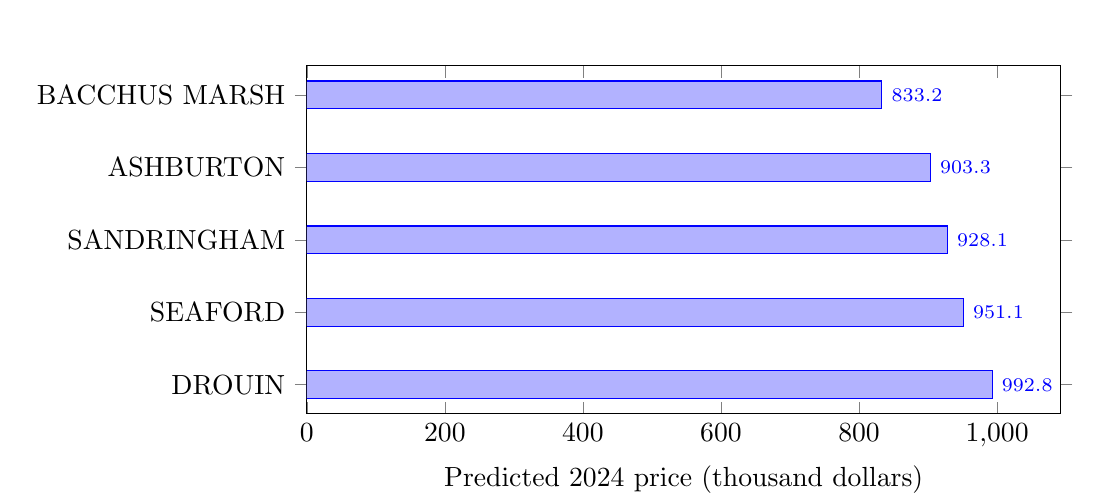
\begin{tikzpicture}
\begin{axis}[
    xbar,
    width=0.92\textwidth,
    height=6cm,
    xlabel={Predicted 2024 price (thousand dollars)},
    ytick={0,1,2,3,4},
    yticklabels={DROUIN,SEAFORD,SANDRINGHAM,ASHBURTON,BACCHUS MARSH},
    xmin=0,
    nodes near coords,
    nodes near coords style={font=\scriptsize},
    fill=orange
]
\addplot coordinates {
(992.8,0)
(951.1,1)
(928.1,2)
(903.3,3)
(833.2,4)
};
\end{axis}
\end{tikzpicture}
\caption{Top predicted price levels show DROUIN first, while SEAFORD remains a strong recommendation because of its larger relative uplift.}
\end{figure}

\section*{Predicted ranking}

\begin{tabular}{lrrr}
\toprule
Suburb & Current price & Predicted 2024 price & Predicted uplift \\
\midrule
DROUIN & 667,824 & 992,801 & 48.7\% \\
SEAFORD & 490,411 & 951,068 & 93.9\% \\
SANDRINGHAM & 577,191 & 928,143 & 60.8\% \\
ASHBURTON & 630,872 & 903,269 & 43.2\% \\
BACCHUS MARSH & 595,045 & 833,151 & 40.0\% \\
\bottomrule
\end{tabular}

\section*{High-uplift candidates}

\begin{tabular}{lrrr}
\toprule
Suburb & Current price & Predicted 2024 price & Predicted uplift \\
\midrule
MONTROSE & 67,157 & 245,452 & 265.5\% \\
WARRNAMBOOL & 64,894 & 221,812 & 241.8\% \\
COBRAM & 73,039 & 229,315 & 214.0\% \\
COLLINGWOOD & 85,746 & 251,603 & 193.4\% \\
AIRPORT WEST & 85,604 & 246,919 & 188.4\% \\
RYE & 110,376 & 267,105 & 142.0\% \\
TEMPLESTOWE & 112,749 & 269,466 & 139.0\% \\
IRYMPLE & 116,905 & 263,180 & 125.1\% \\
\bottomrule
\end{tabular}

\section*{R code appendix}

\begin{lstlisting}[style=rcode]
library(tidyverse)

prices <- read_csv("Data/d01.csv", show_col_types = FALSE) %>%
  mutate(Median_price_2023 = parse_number(Median_price_2023))

hist <- read_csv("Data/d02.csv", show_col_types = FALSE) %>%
  mutate(
    Historical_median_income = replace_na(
      Historical_median_income,
      median(Historical_median_income, na.rm = TRUE)
    ),
    Historical_unemployment_rate_clean = pmax(Historical_unemployment_rate, 0)
  )

proj <- read_csv("Data/d03.csv", show_col_types = FALSE) %>%
  mutate(
    Projected_median_income = replace_na(
      Projected_median_income,
      median(Projected_median_income, na.rm = TRUE)
    ),
    Projected_unemployment_rate_clean = pmax(Projected_unemployment_rate, 0)
  )

analysis_data <- prices %>%
  inner_join(hist, by = "Suburb_name")

model_data <- analysis_data %>%
  filter(Median_price_2023 < 1000000) %>%
  mutate(
    log_price = log(Median_price_2023),
    income_10k = Historical_median_income / 10000
  )

ggplot(analysis_data, aes(x = Median_price_2023)) +
  geom_histogram(bins = 30, fill = "#2a9d8f", color = "white") +
  labs(
    title = "Distribution of 2023 median apartment prices",
    x = "Median apartment price in 2023",
    y = "Number of suburbs"
  ) +
  theme_minimal()

ggplot(model_data, aes(x = Historical_population_growth, y = Median_price_2023)) +
  geom_point(alpha = 0.55, color = "#23395d") +
  geom_smooth(method = "lm", se = FALSE, color = "#c45824") +
  labs(
    title = "Population growth and apartment prices",
    x = "Historical population growth",
    y = "Median apartment price in 2023"
  ) +
  theme_minimal()

ggplot(model_data, aes(x = Historical_unemployment_rate_clean, y = Median_price_2023)) +
  geom_point(alpha = 0.55, color = "#23395d") +
  geom_smooth(method = "lm", se = FALSE, color = "#c45824") +
  labs(
    title = "Unemployment and apartment prices",
    x = "Cleaned unemployment rate",
    y = "Median apartment price in 2023"
  ) +
  theme_minimal()

model <- lm(
  log_price ~ Historical_population_growth +
    income_10k +
    Historical_unemployment_rate_clean +
    Historical_priority_growth_area,
  data = model_data
)

summary(model)

projection_input <- proj %>%
  transmute(
    Suburb_name,
    Historical_population_growth = Projected_population_growth,
    income_10k = Projected_median_income / 10000,
    Historical_unemployment_rate_clean = Projected_unemployment_rate_clean,
    Historical_priority_growth_area = Projected_priority_growth_area
  )

predictions <- projection_input %>%
  mutate(
    pred_log_price_2024 = predict(model, newdata = projection_input),
    pred_price_2024 = exp(pred_log_price_2024)
  ) %>%
  left_join(prices, by = "Suburb_name") %>%
  mutate(
    pred_uplift_abs = pred_price_2024 - Median_price_2023,
    pred_uplift_pct = pred_price_2024 / Median_price_2023 - 1
  )

predictions %>%
  arrange(desc(pred_price_2024)) %>%
  select(Suburb_name, Median_price_2023, pred_price_2024, pred_uplift_pct) %>%
  head(10)

predictions %>%
  filter(Median_price_2023 < 1000000) %>%
  arrange(desc(pred_uplift_pct)) %>%
  select(Suburb_name, Median_price_2023, pred_price_2024, pred_uplift_pct) %>%
  head(15)

top_predictions <- predictions %>%
  filter(Suburb_name %in% c("DROUIN", "SEAFORD", "SANDRINGHAM", "ASHBURTON", "BACCHUS MARSH"))

ggplot(top_predictions, aes(x = reorder(Suburb_name, pred_price_2024), y = pred_price_2024)) +
  geom_col(fill = "#2a9d8f") +
  coord_flip() +
  labs(
    title = "Top predicted apartment prices for next year",
    x = "Suburb",
    y = "Predicted 2024 price"
  ) +
  theme_minimal()

\end{lstlisting}

\end{document}
